\begin{equation}
    \Gamma(s + 1) = \int\limits_0^{\infty} e^{- x} x^s \, dx
	\label{equ:gamma_function}
\end{equation}


\begin{wrapfigure}{r}{0.4\textwidth}
	\centering
	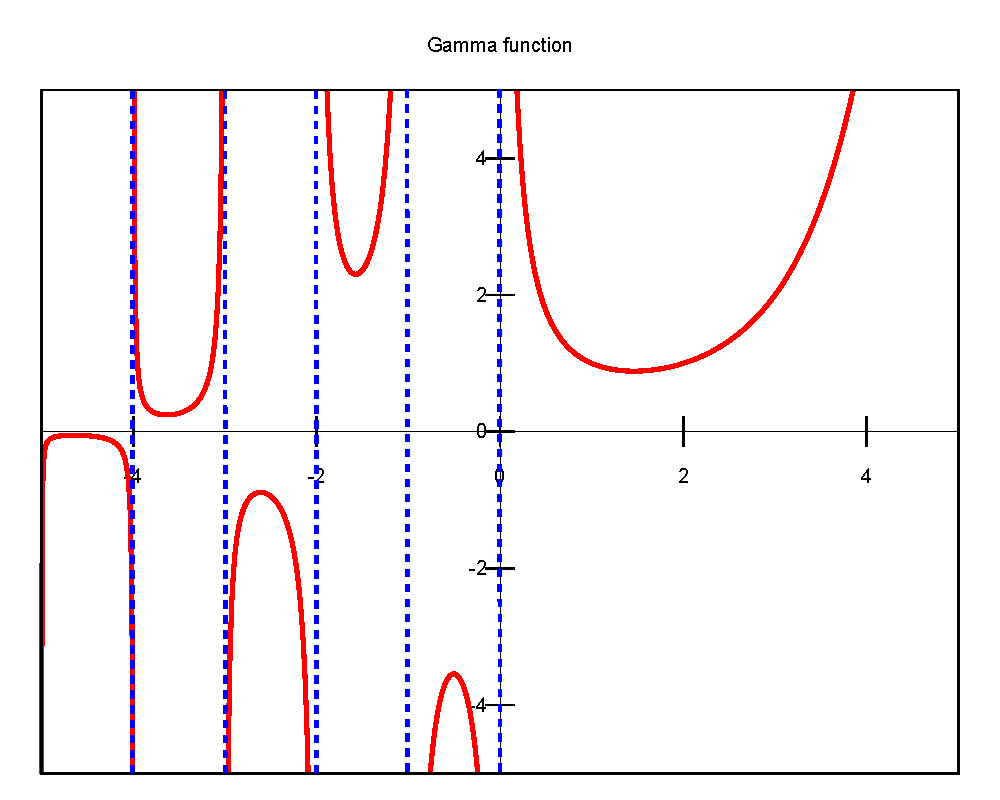
\includegraphics[width=0.4\textwidth]{Gamma_plot.pdf}

\end{wrapfigure}


Функция \eqref{equ:gamma_function} -- гамма-функция.\\
\textbf{Свойства:}
\begin{itemize}
	\item $\displaystyle\Gamma(1 - s) \Gamma(s) = \frac{\pi}{\sin \pi s}$
	\item $\displaystyle\Gamma\left(\frac{1}{2} \right) = \sqrt{\pi}$
	\item $\displaystyle\Gamma(s + 1) = s \Gamma(s)$
	\item  $\displaystyle \Gamma'(x) = \psi(x) \Gamma(x)$ 
	%\item $\displaystyle B(x, y) = \frac{\Gamma(x) \Gamma(y)}{\Gamma(x + y)}$
\end{itemize}
Проинтегрируем по частям
\[
    \Gamma(s + 1) = - e^{-x} x^s |_0^{\infty} + \int\limits_0^{\infty} e^{-x} s x^{s - 1} \, dx = s \int\limits_0^{\infty} e^{-x} x ^{s - 1} \, dx
\]\\

\[
    \Gamma(1) = \int\limits_0^{\infty} e^{- x} x^0 \, dx = \int\limits_0^{\infty} e^{-x} \, dx = \left. e^{- x} \right|_0^{\infty} = 1
\]
\vspace{0.2in}
\[
    \Gamma \left(- \frac{1}{2} + 1\right) = \int\limits_0^{\infty} e^{-x} x^{- \frac{1}{2}} \, dx \left[ \begin{tabular}{c c} $x = z^2$ & $\sqrt{x} = z$\\ $dx = 2z dz$& \end{tabular} \right] = \int\limits_0^{\infty} \frac{e^{-z^2}}{z} 2 z \, dz = 2 \int\limits_0^{\infty} e^{-z^2} \, dz =\sqrt{\pi}
\]

\[
    \Gamma(1) = 1 \quad \Gamma\left(\frac{1}{2}\right) = \sqrt{\pi}
\]

\[
    \Gamma\left(\frac{3}{2}\right) = \Gamma\left(\frac{1}{2} + 1\right) = \frac{1}{2} \Gamma\left(\frac{1}{2}\right) = \frac{\sqrt{\pi}}{2}
\]

Гамма-функции встречаются в уравнениях Бесселя.



